\section{Concurrency}
\subsubsection{Lost Update}
\begin{itemize}
    \item Eine Transaktion überschreibt die Änderungen einer anderen:
    \item Es wird der Wert ausgelesen, bevor die 2. Transaktion beginnt!
\end{itemize}
\begin{figure}[H]
    \centering
    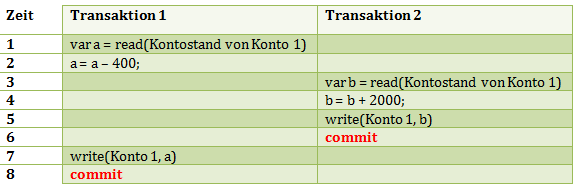
\includegraphics{res/themenkorb_5/lostupdate.png}
\end{figure}
\subsubsection{Dirty Read}
\begin{itemize}
    \item Kommt nur in Zusammenhang mit Rollback vor!
    \item Eine Transaktion liest Werte von einer anderen, welche im Nachinein wieder rückgängig (Rollback) gemacht wird!
\end{itemize}
\begin{figure}[H]
    \centering
    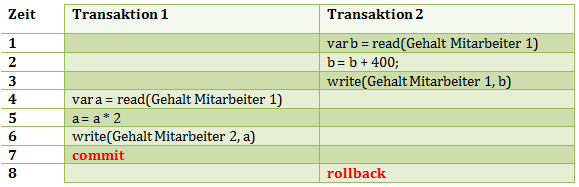
\includegraphics{res/themenkorb_5/dirtyread.png}
\end{figure}
\subsubsection{Non-Repeatable Read}
\begin{itemize}
    \item Entsteht dann, wenn lesende Vorgänge von einer anderen Transaktion unterbrochen werden!
    \item Beim nächsten Read liefert die Abfrage dann andere Ergebnisse, da hier keine 2. Transaktion "dazwischenpfuscht"!
\end{itemize}
\begin{figure}[H]
    \centering
    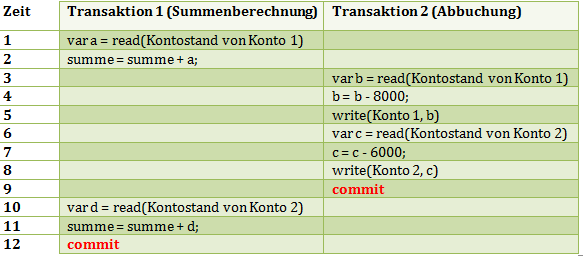
\includegraphics{res/themenkorb_5/nonrepeatableread.png}
\end{figure}
\subsubsection{Phantom}
\begin{itemize}
    \item Kommt meist im Zusammenhang mit Aggregatfunktionen vor, wenn sich z.B. durch eine andere Transaktion die Anzahl an Record ändert!
\end{itemize}
\begin{figure}[H]
    \centering
    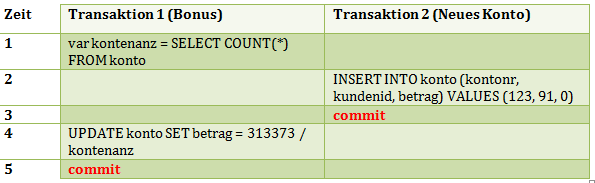
\includegraphics{res/themenkorb_5/phantom.png}
\end{figure}

\subsection{Serialisierbarkeit}
\begin{itemize}
    \item Als serialisierbar wird ein Ausführungsplan (Gibt an, welche Transaktion ausgeführt wird) dann bezeichnet, wenn das Ergebnis das selbe als jenes eines seriellen Ablaufes ist
    \item Überprüfung von Serialisierbarkeit $\implies$ Es wird ein Graph mit allen Operation aufgebaut; wenn dieser keinen Cycle enthält $\implies$ Serialisierbar (In gewisser Reihenfolge)!
\end{itemize}

\subsection{Lösungsmöglichkeiten}
\subsubsection{Sperrverfahren}
\begin{itemize}
    \item Pessimistisch
    \begin{itemize}
        \item Es wird davon ausgegangen, dass Konflikte auftreten $\implies$ Objekte werden von Anfang an gesperrt
    \end{itemize}
    \item Optimistisch
    \begin{itemize}
        \item Es wird davon ausgegangen, dass keine Probleme auftreten $\implies$ Falls doch, muss die Datenbank reagieren!
    \end{itemize}
    \item Timestamp
    \begin{itemize}
        \item Jede Transaktion enthält Startzeitpunkt $\implies$ Konflikt tritt auf, wenn jüngere Transaktion die gleichen Daten beschreibt!
    \end{itemize}
\end{itemize}
\subsubsection{Sperrebenen}
\begin{itemize}
    \item Je feiner, desto aufwändiger, aber höhere Parallelität
    \item Je gröber, desto leichter, aber geringere Parallelität
    \item Ebenen
    \begin{itemize}
        \item Datenbank
        \item Tabelle
        \item Physischer Block / Seite
        \item Zeile
    \end{itemize}
\end{itemize}
\subsubsection{Arten von Sperren}
\begin{itemize}
    \item X-Lock $\implies$ Exklusiv, Read/Write erlaubt; es können keine weiteren Locks gesetzt werden!
    \item S-Lock $\implies$ Shared, Read erlaubt; es können weitere S-Locks gesetzt werden!
\end{itemize}

\subsection{Deadlocks}
\begin{itemize}
    \item Tritt dann auf, wenn 2 Transaktionen sich gegenseitig behindern (beide warten darauf, einen Lock auf gewisse Daten zu setzen!)!
    \item z.B. Wenn beide einen S-Lock auf einen Datensatz haben und dann jeweils einen X-Lock auf die anderen Daten setzen wollen
\end{itemize}
\subsubsection{Behandlung}
\begin{itemize}
    \item Vermeidung
    \begin{itemize}
        \item Eine Transaktion wird abgebrochen, wenn bei einer Sperranforderung die Gefahr auf einen Deadlock besteht; es werden sämtliche benötigte Objekte von Anfang an gesperrt!
    \end{itemize}
    \item Erkennung
    \begin{itemize}
        \item Es wird ein (gerichteter) Wartegraph geführt
        \begin{itemize}
            \item Knoten $\implies$ Die einzelnen Transaktionen
            \item Kanten $\implies$ Werden zwischen 2 Knoten gezeichnet, wenn einer auf den anderen warten muss
            \item Deadlock ist dann vorhanden, wenn im Graphen Zyklen enthalten sind!
        \end{itemize}
        \begin{figure}[H]
            \centering
            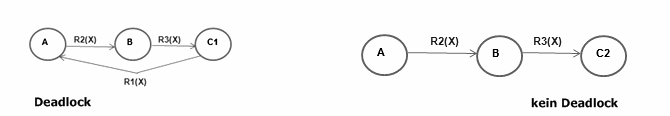
\includegraphics[width=\textwidth]{res/themenkorb_5/ein_kein_deadlock.png}
        \end{figure}
    \end{itemize}
\end{itemize}

\subsection{Re-Read Methode}
\begin{itemize}
    \item Wird bei Änderungen an Daten im Mehruserbetrieb verwendet
    \item Ablauf
    \begin{enumerate}
        \item Daten einlesen (ohne Sperre) $\implies$ Record-Old
        \item Daten (oder Teile) von Record-Old kopieren $\implies$ Record-Update
        \item Daten in Record-Update (oder Teile davon) vom Benutzer ändern lassen
        \item Datensatz erneut einlesen (mit X-Lock) $\implies$ Record-Check
        \item Record-Check mit Record-Old vergleichen:
        \begin{enumerate}
            \item Gleich $\implies$ Update zulässig
            \item Ungleich $\implies$ Update unzulässig
        \end{enumerate}
    \end{enumerate}
\end{itemize}

\subsection{U-Lock}
\begin{itemize}
    \item Kann bei Leseoperationen angegeben werden, um anschließend beabsichtigte Änderungs Operationen anzuzeigen
\end{itemize}

\subsection{Isolation-Levels}
\begin{itemize}
    \item Read Uncommitted
    \begin{itemize}
        \item kein Lock beim Lesen
        \item Dirty Read, Non-Repeatable Read + Phantom sind möglich
    \end{itemize}
    \item Read Committed
    \begin{itemize}
        \item S-Lock auf Zeile beim Lesen, kein Two-Phase Locking
        \item Non-Repeatable Read + Phantom sind möglich
    \end{itemize}
    \item Repeatable Read
    \begin{itemize}
        \item S-Lock auf Zeile beim Lesen bis Transaktionsende
        \item Phantom ist möglich
    \end{itemize}
    \item Serializable
    \begin{itemize}
        \item S-Lock auf \textbf{Tabelle} beim Lesen bis Transaktionsende oder Predicate Locking
        \item Nichts ist möglich
    \end{itemize}
\end{itemize}